\documentclass{beamer}
\usetheme[pageofpages=of,% String used between the current page and the
                         % total page count.
          bullet=circle,% Use circles instead of squares for bullets.
          titleline=true,% Show a line below the frame title.
          alternativetitlepage=true,% Use the fancy title page.
       %   titlepagelogo=logo-polito,% Logo for the first page.
       %   watermark=watermark-polito,% Watermark used in every page.
       %   watermarkheight=100px,% Height of the watermark.
       %   watermarkheightmult=4,% The watermark image is 4 times bigger
                                % than watermarkheight.
          ]{Torino}

\setbeamertemplate{footline}{
  \begin{beamercolorbox}[wd=\paperwidth,ht=1ex,dp=1ex]{footline}
    \vspace{5pt} \hspace{1em} \insertframenumber/\inserttotalframenumber
  \end{beamercolorbox}
}

\author{Brendon J. Brewer}
\title{STATS 331 -- Introduction to Bayesian Statistics}
\institute{The University of Auckland}
\date{}


\linespread{1.3}
\usepackage{minted}
\usepackage[utf8]{inputenc}
\usepackage{dsfont}
\newcommand{\given}{\,|\,}
\newcommand{\balpha}{\boldsymbol{\alpha}}
\newcommand{\bmu}{\boldsymbol{\mu}}


\begin{document}

\frame{\titlepage}

\begin{frame}
\Large

\begin{center}
Review
\end{center}
\end{frame}

\begin{frame}
\frametitle{Lecture Purpose}

We will now briefly review the course content, and I will outline my
expectations for what you should be able to do in the exam.

\end{frame}

\begin{frame}
\frametitle{SET Evaluations}
Please do them!

\end{frame}


\begin{frame}
\frametitle{Probabilities}
The mathematics of {\bf probabilities} can be used to describe two different
things: proportions, and uncertainties. Which interpretation you adopt
determines the way you end up using the maths.\pause

   \begin{columns} % Create two columns

        \column{0.5\textwidth} % Left column (50% width)
        \centering
        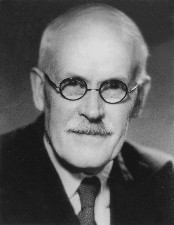
\includegraphics[width=0.5\linewidth]{images/jeffreys.jpg}

        Harold Jeffreys (Bayesian)

        \column{0.5\textwidth} % Right column (50% width)
        \centering
        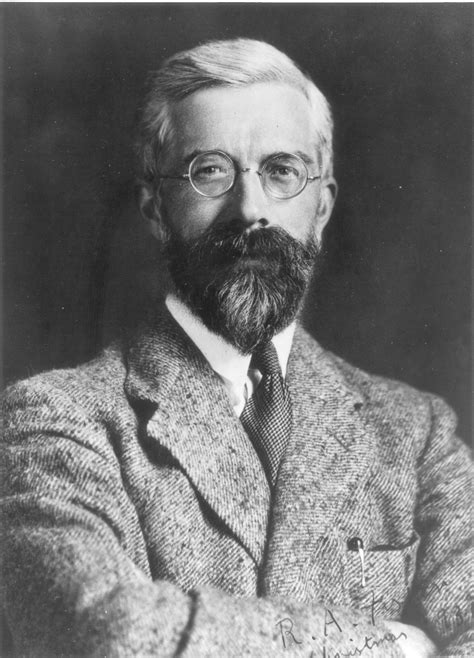
\includegraphics[width=0.5\linewidth]{images/fisher.jpg}

        R. A. Fisher (Frequentist)
     \end{columns}


\end{frame}


\begin{frame}
\frametitle{Rules of Probability}
Fundamentally, there are two rules of probability, the sum rule and the
product rule. Their most general versions are given below.

\begin{align}
P(A \vee B \given C) &= P(A \given C) + P(B \given C) - P(A, B \given C) \\
P(A, B \given C) &= P(A \given C)P(B \given A, C).
\end{align}\pause

Other rules such as Bayes' rule and the partition theorem are derived from
these.


\end{frame}


\begin{frame}
\frametitle{Sum Rule Applications}
The sum rule shows up in Bayesian statistics in a few different situations:\pause

\begin{itemize}
\item Prior and posterior probabilities of `OR' statements (a popular exam
question that is easy marks).\pause
\item Marginal likelihood calculation.\pause
\item Predictions.\pause
\item Finding marginal posterior distributions (for one parameter only)
from joint distributions (of more than one parameter).
\end{itemize}


\end{frame}


\begin{frame}
\frametitle{Product Rule Applications}
The product rule shows up in Bayesian statistics in a few different situations:\pause

\begin{itemize}
\item Bayes' rule, used for updating probabilities, comes from the product
rule.\pause
\item Joint distributions are formed using the product rule. This is how
we can construct prior distributions for more than one parameter, or
sampling distributions for more than one data value.
\end{itemize}


\end{frame}


\begin{frame}
\frametitle{Bayes' Rule}
The most important form of Bayes' rule is the one that gives you the
posterior probabilities of some mutually exclusive hypotheses $H_i$:

\begin{align}
P(H_i \given D) &= \frac{P(H_i)P(D \given H_i)}{P(D)}
\end{align} \pause
where
\begin{align}
P(D) &= \sum_i P(H_i) P(D \given H_i).
\end{align}


\end{frame}


\begin{frame}
\frametitle{Checklist for Exam}

\begin{itemize}
\item Ideally, know these rules from memory (but you can use your cheat sheet
too).\pause
\item Know how to do a Bayes Box. Part of this is being able to read the
question and to know what values go in the prior
and likelihood columns of the Bayes Box.\pause
\item Be able to write down Bayes' rule or the marginal likelihood formula
corresponding to the particular statements in a given problem.
\end{itemize}


\end{frame}

\begin{frame}
\frametitle{Exam Hint}
Question 1 (out of 4) is a Bayes Box question. One of the parts, which is
about calculating the posterior probabilities, is worth 10\% of the total
marks. I expect most people to answer that correctly.\pause

Don't forget a calculator, as I did not ensure that all the results are
nice fractions.

\end{frame}


\begin{frame}
\frametitle{Parameter Estimation}
Recall that Bayes' rule can be used on a set of mutually exclusive hypotheses.
These can be statements about the value of the parameter $\theta$.\pause

\begin{itemize}
\item One hypothesis might be ``$\theta = 1$'' \pause
\item Another might be ``$\theta = 2$'' \pause
\item We might get some data like ``$x = 3$''.
\end{itemize}

\end{frame}


\begin{frame}
\frametitle{Bayes' Rule Lots of Times}
\begin{align}
P(\theta = 1 \given x = 3) &= \frac{P(\theta=1)P(x=3 \given \theta=1)}{P(x=3)}\\
P(\theta = 2 \given x = 3) &= \frac{P(\theta=2)P(x=3 \given \theta=2)}{P(x=3)}\\
&...&\\
P(\theta = 9 \given x = 3) &= \frac{P(\theta=9)P(x=3 \given \theta=9)}{P(x=3)}\\
\end{align}

\end{frame}

\begin{frame}
\frametitle{Bayes' Rule Lots of Times}
\begin{align}
\color{red}{P(\theta = 1 \given x = 3)} &= \frac{{\color{blue}P(\theta=1)}P(x=3 \given \theta=1)}{P(x=3)}\\
\color{red}{P(\theta = 2 \given x = 3)} &= \frac{{\color{blue}P(\theta=2)}P(x=3 \given \theta=2)}{P(x=3)}\\
&...&\\
\color{red}{P(\theta = 9 \given x = 3)} &= \frac{{\color{blue}P(\theta=9)}P(x=3 \given \theta=9)}{P(x=3)}\\
\end{align}

{\color{red}Posterior Distribution}
{\color{blue}Prior Distribution}

\end{frame}


\begin{frame}
\frametitle{Bayes' Rule Lots of Times}
\begin{align}
P(\theta = 1 \given x = 3) &= \frac{P(\theta=1){\color{orange}P(x=3 \given \theta=1)}}{\color{green}P(x=3)}\\
P(\theta = 2 \given x = 3) &= \frac{P(\theta=2){\color{orange}P(x=3 \given \theta=2)}}{\color{green}P(x=3)}\\
&...&\\
P(\theta = 9 \given x = 3) &= \frac{P(\theta=9){\color{orange}P(x=3 \given \theta=9)}}{\color{green}P(x=3)}\\
\end{align}

{\color{orange}Likelihood Function}
{\color{green}Marginal Likelihood (common to all $\theta$ values)}

\end{frame}

\begin{frame}
\frametitle{Bayes Box for Parameter Estimation}
Since a Bayes Box is equivalent to these repeated uses of Bayes' rule,
we can use Bayes Boxes for parameter estimation (when there is only one unknown
parameter).\pause

I expect you to know the R code for this. I might ask you to read some
code that does this and fill in a missing line or two, or to write down the
line that you would need to do some sort of post-processing.

\end{frame}

\begin{frame}
\frametitle{R Code in the Exam}
There will usually be one or two parts, worth a few percent, where I ask you
to read or write a little bit of R code. Not too extensive, as this is not
a programming course.\pause\\[1em]

If you do not know the exact R code, but have the right idea, you can still
get part marks, so don't feel bad about writing something down if you think
it might not be perfectly correct.

\end{frame}


\begin{frame}
\frametitle{Plots in the Exam}
Plots may or may not show up in the exam. Sometimes I ask you to:
\begin{itemize}
\item Interpret what you see in a given plot.\pause
\item Sketch how you would expect a certain plot to look.\pause
\end{itemize}
If I ask you to sketch a plot, you probably won't get many marks for the
bare minimum effort (e.g., drawing a bell curve for the posterior distribution).
In that case you would get full marks if you labelled the axes and put some values
showing what you think $\theta$ would be, for instance.

\end{frame}


\begin{frame}
\frametitle{Bayes' Rule for Parameter Estimation}
We have written this down in a few different forms:

\begin{align}
p(\theta \given x) &= \frac{p(\theta)p(x\given \theta)}{p(x)} \\
p(\theta \given x) &\propto p(\theta)p(x\given \theta) \\
\texttt{posterior} &\propto \texttt{prior} \times \texttt{likelihood}.
\end{align}

\end{frame}

\begin{frame}
\frametitle{Analytical Methods}
We spent about 1.5 lectures on analytical methods, but they are quite important
(even though we only looked at the basics). In 331 we focused on
\begin{align}
p(\theta \given x) &\propto p(\theta)p(x\given \theta)
\end{align}
for particular situations that work out with a recognisable distribution
for the posterior $p(\theta \given x)$. Mostly these are with conjugate priors.
\end{frame}


\begin{frame}
\frametitle{Conjugate Priors}

\begin{itemize}
\item Binomial sampling distribution + Beta prior $\implies$ Beta posterior \pause
\item Poisson sampling distribution + Gamma prior $\implies$ Gamma posterior \pause
\item Multinomial sampling distribution + Dirichlet prior $\implies$ Dirichlet posterior.
\end{itemize}
\pause
Also, special cases of these, for example when the Beta prior is a Beta$(1, 1)$
(aka Uniform$(0, 1$)), you still get a Beta posterior.

\end{frame}

\begin{frame}
\frametitle{Exam Hint}
Question 2 of the exam has you computing the posterior distribution for one
of these cases, recognising what it is, writing it in ``$\sim$'' notation,
and computing one or two summaries from it.\\[0.5em]\pause

I also expect you to be able to write down the likelihood function, which
is one of the steps in getting to the posterior distribution. Remember that
for multiple data values the likelihood function involves a product of terms,
one for each data point.

\end{frame}


\begin{frame}
\frametitle{Formula Sheet}
In the exam, a formula sheet will be provided, which has some properties of
a few distributions. This will be the same formula sheet from the test.
Don't waste space or time putting these formulas on your cheat sheet (unless
you think it will help you in applying them).

\end{frame}


\begin{frame}
\frametitle{Hypothesis Testing/Model Selection}
We spent some time discussing hypothesis testing and model selection,
mostly in one dimension (one unknown parameter). What should you know?\pause

\begin{itemize}
\item Spike-and-slab prior: what it is for, how to make one, how to interpret
the results.\pause
\item I am quite fond of asking questions about how the results depend on the
shape and/or width of the slab, and not just on the height of the spike.\pause
\item Know how to express conclusions as posterior probabilities, odds ratios,
or Bayes factors, and how to convert between these.
\end{itemize}


\end{frame}


\begin{frame}
\frametitle{Prediction}
I would like you to understand how Bayesian prediction works, but you should
only expect a small amount of it to show up on the exam.

\centering
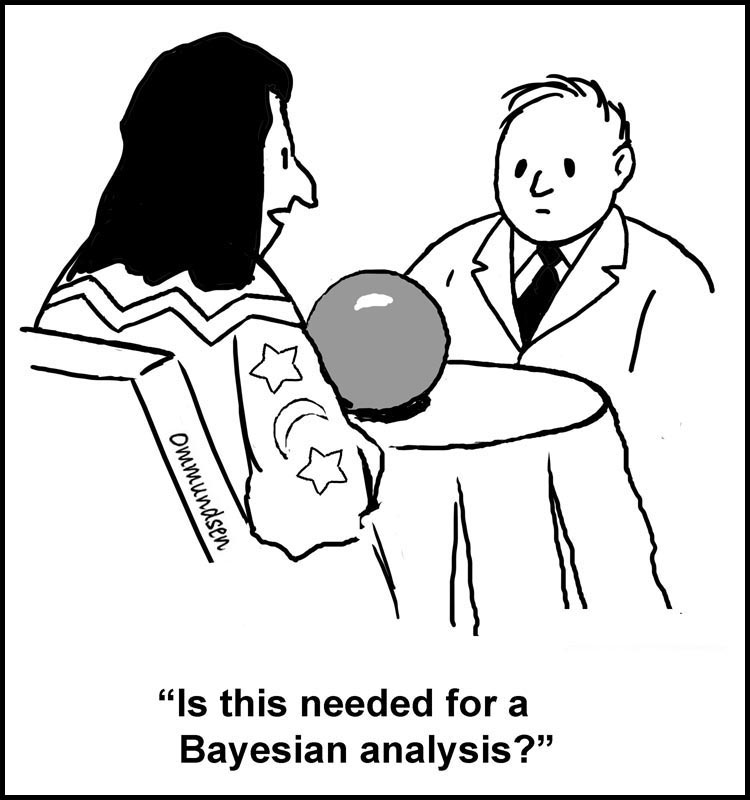
\includegraphics[width=0.35\textwidth]{images/crystal_ball.jpg}

\end{frame}

\begin{frame}
\frametitle{Prediction}

\begin{itemize}
\item Know the basic principle of it --- that you first make the predictions
under the assumption that you know $\theta$, then you take the posterior
expectation/mean of the result. \pause
\item Know how to do it in simple cases (e.g. a Bayes Box type question).\pause
\item Know how to do it in JAGS (adding extra node(s) for the predicted future
data).
\end{itemize}



\end{frame}


\begin{frame}
\frametitle{Summaries}
We looked at how to summarise posterior distributions.

\begin{itemize}
\item You can just compute simple summaries like posterior mean and
standard deviation to give an idea of the location and width of the
posterior distribution.\pause
\item We studied decision theory which can give an idea of what kind of
point estimate is `best', but it depends on what kind of loss function you
think is reasonable. Remember the three cases of loss functions that
lead to posterior mean, median, and mode being optimal. \pause
\item Credible intervals.
\end{itemize}

\end{frame}


\begin{frame}
\frametitle{R Code Again}

There is some chance I will ask questions like `write down the R code you would
use to compute a particular summary' (after having shown you the R code for
calculating the posterior distribution itself).\pause\\[0.5em]

Or, I might show you some code and its output, and expect you to know which
bit is doing the thing I want you to talk about.
\end{frame}




\begin{frame}
\frametitle{Intervals}
Not many people understand the difference between a credible interval and
a confidence interval.\pause

\begin{itemize}
\item Credible interval: Given the data, there is a 95\% chance (or whatever)
that the parameter is in the interval. {\bf Based on the posterior distribution}.\pause
\item Confidence interval: This particular way of producing intervals will
contain the parameter for 95\% of possible datasets.
{\bf Based on the sampling distribution as frequentist theory doesn't have
posterior distributions in it}.
\end{itemize}

\end{frame}


\end{document}

